\documentclass[a4paper,12pt]{article}
\usepackage{xcolor}
\usepackage{amsmath,amsfonts,amssymb}
\usepackage{geometry}
\usepackage{fancyhdr}
\usepackage{graphicx}
\usepackage{titlesec}
\usepackage{tikz}
\usepackage{booktabs}
\usepackage{array}
\usetikzlibrary{shadows}
\usepackage{tcolorbox}
\usepackage{float}
\usepackage{lipsum}
\usepackage{mdframed}
\usepackage{pagecolor}
\usepackage{mathpazo}   % Palatino font (serif)
\usepackage{microtype}  % Better typography

\setlength{\parindent}{0pt}

% Page background color
\pagecolor{gray!10!white}

% Geometry settings
\geometry{margin=0.5in}
\pagestyle{fancy}
\fancyhf{}

% Fancy header and footer
\fancyhead[C]{\textbf{\color{blue!80}CS765 Project Part-1}}
% \fancyhead[R]{\color{blue!80}Saksham Rathi}
\fancyfoot[C]{\thepage}

% Custom Section Color and Format with Sans-serif font
\titleformat{\section}
{\sffamily\color{purple!90!black}\normalfont\Large\bfseries}
{\thesection}{1em}{}

% Custom subsection format
\titleformat{\subsection}
{\sffamily\color{cyan!80!black}\normalfont\large\bfseries}
{\thesubsection}{1em}{}

% Stylish Title with TikZ (Enhanced with gradient)
\newcommand{\cooltitle}[1]{%
\begin{tikzpicture}
\node[fill=blue!20,rounded corners=10pt,inner sep=12pt, drop shadow, top color=blue!50, bottom color=blue!30] (box)
{\Huge \bfseries \color{black} #1};
\end{tikzpicture}
}
\usepackage{float} % Add this package

\newenvironment{solution}[2][]{%
\begin{mdframed}[linecolor=blue!70!black, linewidth=2pt, roundcorner=10pt, backgroundcolor=yellow!10!white, skipabove=12pt, skipbelow=12pt]%
	\textbf{\large #2}
	\par\noindent\rule{\textwidth}{0.4pt}
}{
\end{mdframed}
}

% Document title
\title{\cooltitle{CS765 Project Part-1} \\
\LARGE \textbf{Simulation of a P2P Cryptocurrency Network} \\
Report}
\author{{\bf Saksham Rathi (22B1003), Kavya Gupta (22B1053), Mayank Kumar (22B0933)} \\
\small Department of Computer Science, \\
Indian Institute of Technology Bombay \\}
\date{}

\begin{document}
\maketitle


\begin{solution}{Point 2}
	Theoretical reasons of choosing the exponential distribution for
	interarrival time sampling are:-
	\begin{itemize}
		\item The most important theoretical reason for using the exponential distribution for inter-arrival times is its \textbf{memoryless property}, which means that the probability of an event occurring in the future is independent of the past. Specifically:
		\begin{equation*}
			P(X > s + t | X > s) = P(X > t)
		\end{equation*}
		This is particularly helpful as this makes the future transactions independent of the past which is true as all transactions are independently randomly generated.
		\item It's \textbf{correspondence to the Poisson} distribution. The Poisson distribution is about the most basic count process, with constant event rate and no memory. This can help model the generation of transactions appropriately. Whenever a Poisson models the distribution of events then an Exponential models the distribution of inter-event times.
	\end{itemize}
\end{solution}

\begin{solution}{Point 5}
	The mean of $d_{i,j}$ (queuing delay) is inversely related to $c_{i,j}$ (link speed) because a higher link speed allows messages to be transmitted more quickly, reducing the time they spend in the queue. For example, if a link has higher capacity, it can process and forward packets at a faster rate, reducing the time packets spend in the queue. Conversely, a lower link speed results in congestion, as packets arrive faster than they are transmitted, increasing queuing delays. Therefore delay is inversely proportional to link speed.
\end{solution}

\begin{solution}{Point 7}
	We chose the mean block arrival time (I) as 600 seconds. The reasons for it are as follows:-
	\begin{itemize}
		\item Choosing a very high value would result in a very low number of blocks being generated in the network, which would not be a good representation of a real-world cryptocurrency network. In our simulation, we found out that (for certain parameters) I = 600 sec will have $\approx$ 10 times the longest chain height than I = 60000 sec in half the time. For I = 6000000 sec, the simulation didn't give any meaningful results, due to too many transaction events.
		\item Choosing a very low value would likely lead to many instances of forking, orphaning a lot of blocks and hence a very branched tree. For Ethereum, it is 15 seconds and for that our simulation returns this dense tree:-
		\begin{figure}[H]
			\centering
			\includegraphics[width=0.88\textwidth]{ethereum-case.png}
		\end{figure}
		\item For Bitcoin blockchain, this value is 600 seconds as well, hence choosing this value would be likely provide simulations closer to the actual things.
	\end{itemize}
\end{solution}

\begin{solution}{Flowchart of Event Execution}
	\begin{figure}[H]
		\centering
		\fbox{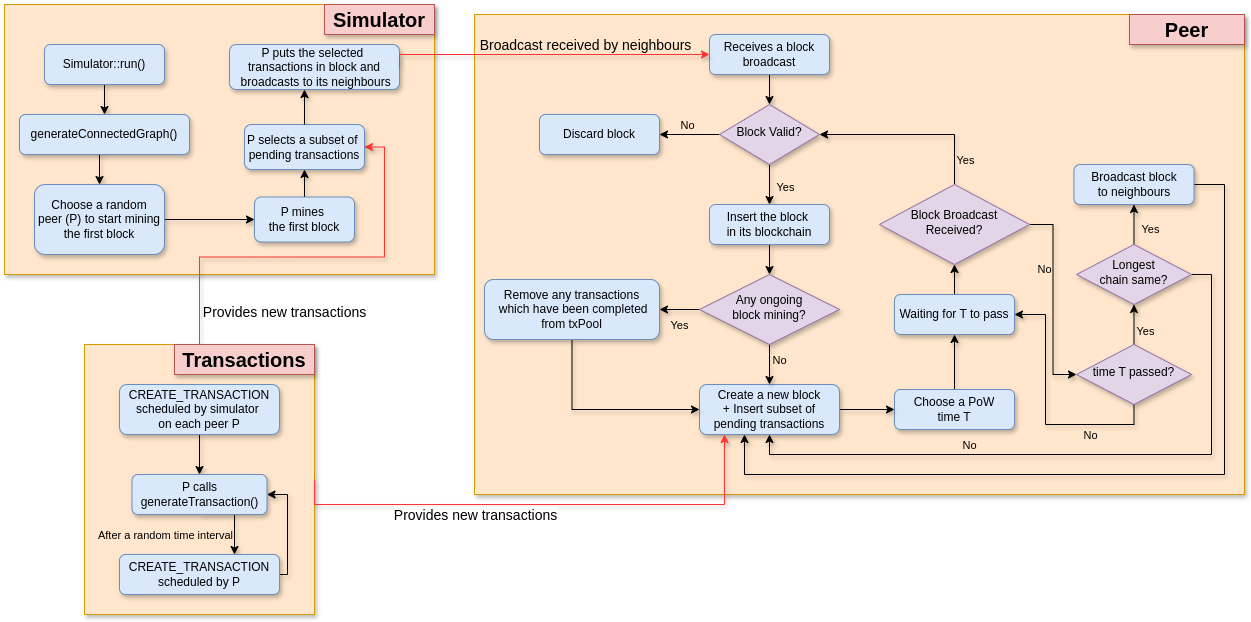
\includegraphics[width=1\textwidth]{../images/flowchart.png}}
		\caption{Flow of events}
	\end{figure}
\end{solution}

\begin{solution}{Analysis}
	We are analyzing the following ratio:
	\begin{equation*}
		\text{Ratio$_i$} = \frac{\text{Total number of transactions in the longest chain from peer $i$}}{\text{Total number of transactions produced by peer $i$ in the network}}
	\end{equation*}

	Here is the default list of parameters which we have chosen for our analysis:
	\begin{itemize}
		\item Number of peers: 100
		\item Percentage of slow peers: 50\%
		\item Percentage of low CPU peers: 50\%
		\item Mean transaction interarrival time: 10 seconds
		\item Mean block arrival time: 600 seconds
	\end{itemize}

	Some general inferences:

	\begin{itemize}
		\item The ratio is higher for fast nodes as compared to the slow nodes. Because, across a link with both fast nodes, the latency is less, and hence the peer nodes are able to communicate their blocks faster. (The blocks which come later are invalid, and hence the ratio is higher for fast nodes).
		\item The ratio is lesser in case of high CPU nodes. Because of their higher hashing power, they complete their mining before the blockchain gets stabilized, and thus produce forks, and a decreased ratio.
	\end{itemize}

	In the graph shown below, we vary one of these parameters and deduce inferences from the graph.
	\begin{figure}[H]
		\centering
		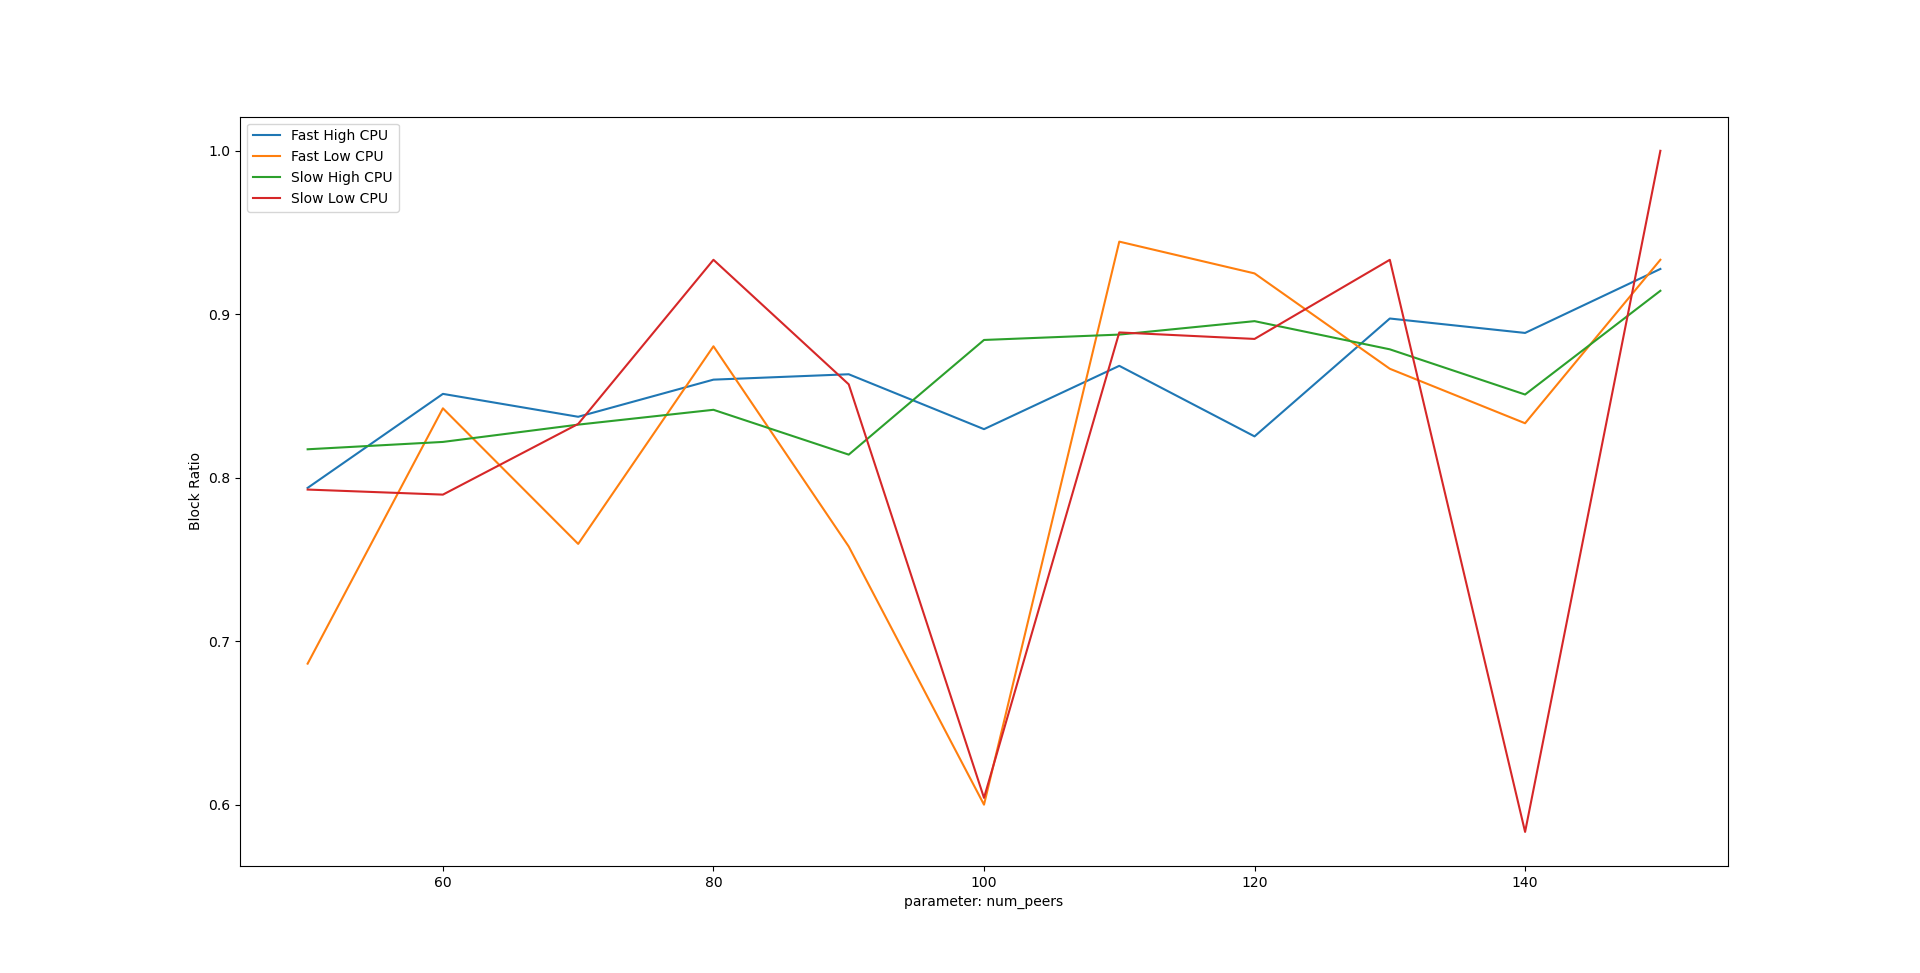
\includegraphics[width=0.8\textwidth]{../images/avg_run_3/num_peers.png}
		\caption{Ratio v/s Number of peers}
		\label{fig:simulation_plot1}
	\end{figure}

	The above is the graph of the ratio across various types of peer nodes vs the number of nodes in the network. The ratio is in general higher for fast nodes as compared to the slow nodes, because across a link where both the nodes are fast nodes, the latency is quite less, and hence the peer nodes are able to communicate their blocks faster. Rest, there are some outliers in the graph too.

	\begin{figure}[H]
		\centering
		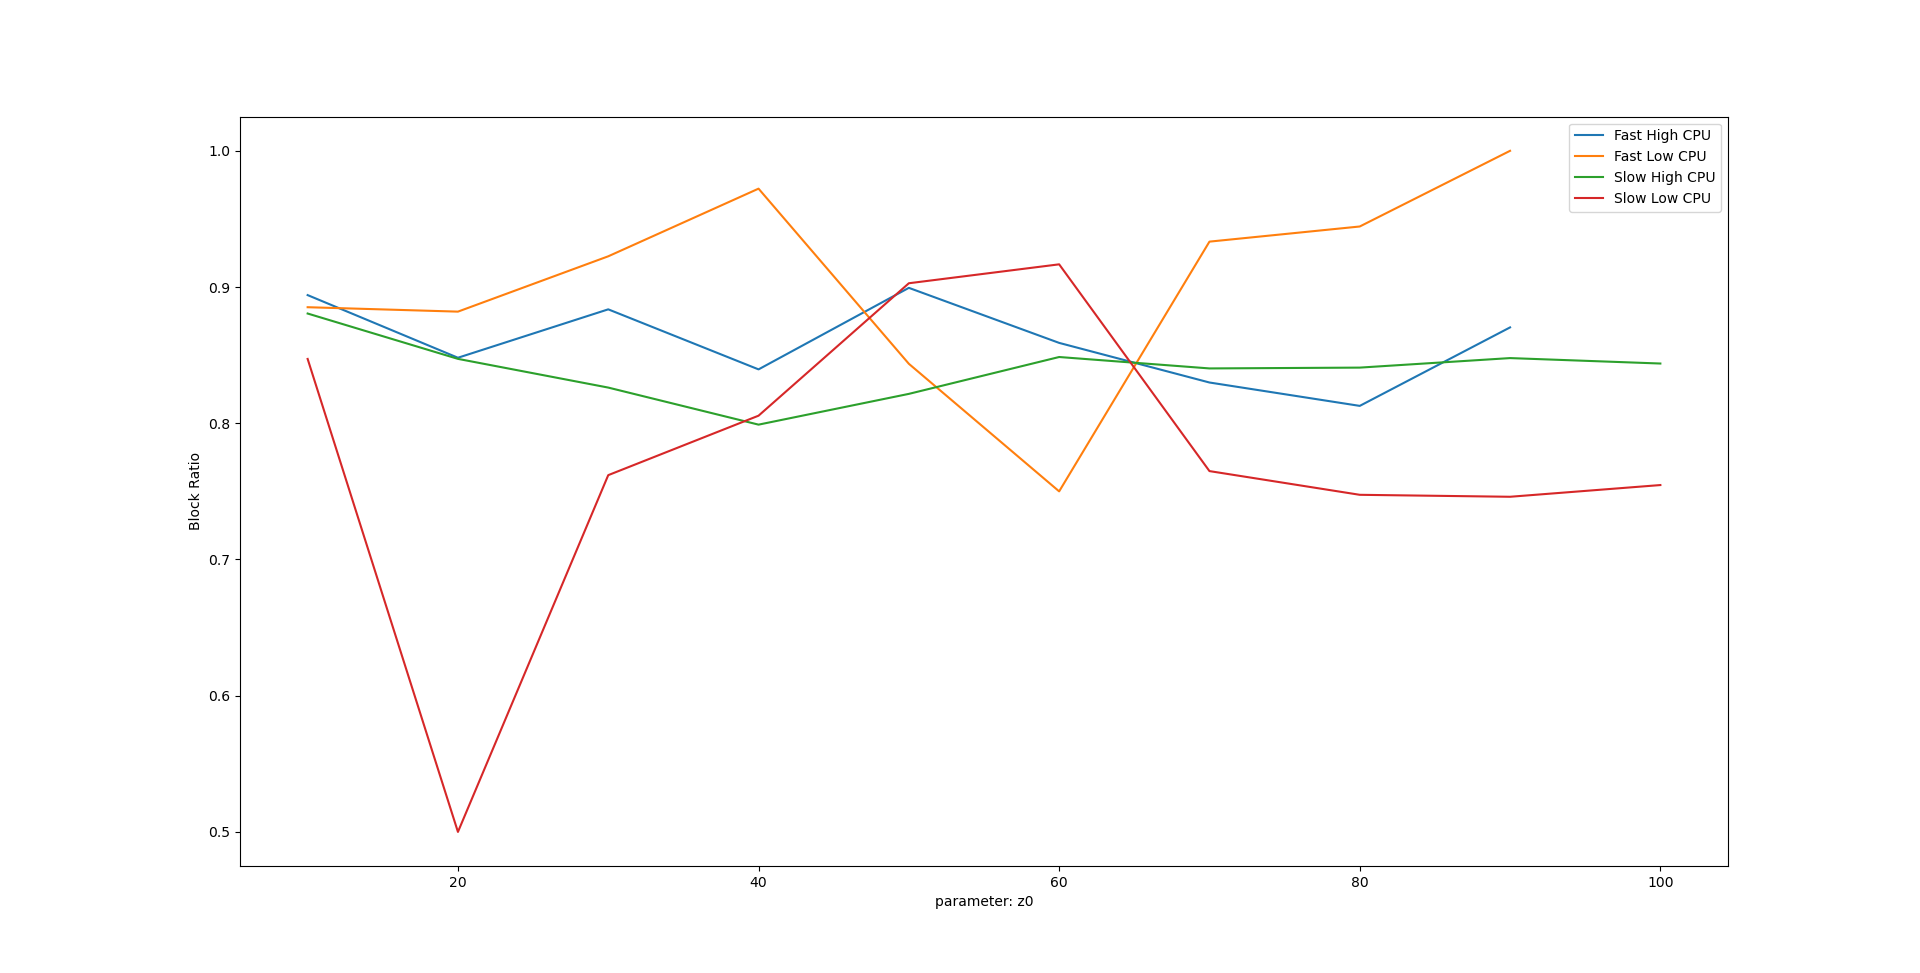
\includegraphics[width=0.8\textwidth]{../images/avg_run_3/z0.png}
		\caption{Ratio v/s Percentage of Slow Peers}
		\label{fig:simulation_plot2}
	\end{figure}

	The above graph is the ratio vs the percentage of slow nodes in the graph. The ratio is again higher for fast nodes. Overall, there is neither an upward nor a downward trend in the graph, which shows that the percentage of slow nodes does not affect the ratio much (for a link to have lower latency, both the nodes need to be fast).

	\begin{figure}[H]
		\centering
		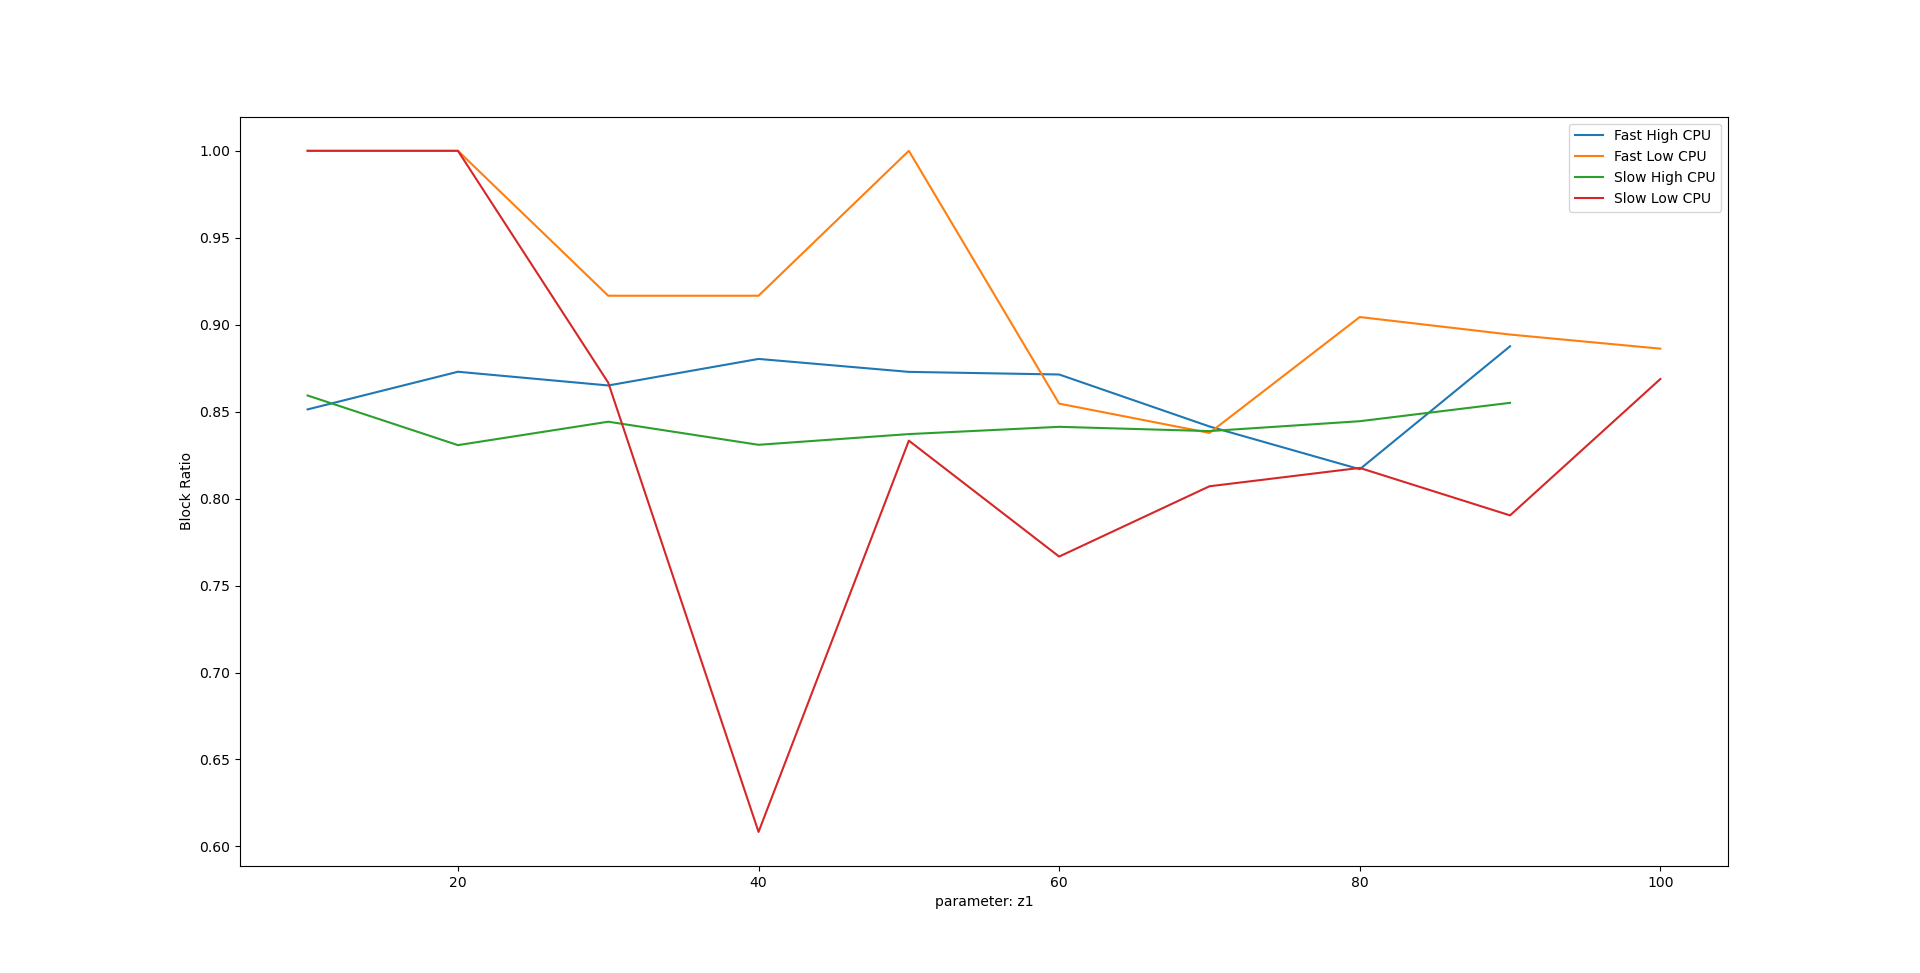
\includegraphics[width=0.8\textwidth]{../images/avg_run_3/z1.png}
		\caption{Ratio v/s Percentage of Low CPU Peers}
		\label{fig:simulation_plot3}
	\end{figure}

	The above graph is the ratio vs the percentage of low CPU nodes in the graph. The ratio is similar across various types of nodes, which shows us that the network which we have created gives proper chance to all types of nodes. However, the number of blocks produced by the fast CPU nodes is higher, and because of similar ratios, the number of blocks in the blockchain is also higher for fast CPU nodes.


	\begin{figure}[H]
		\centering
		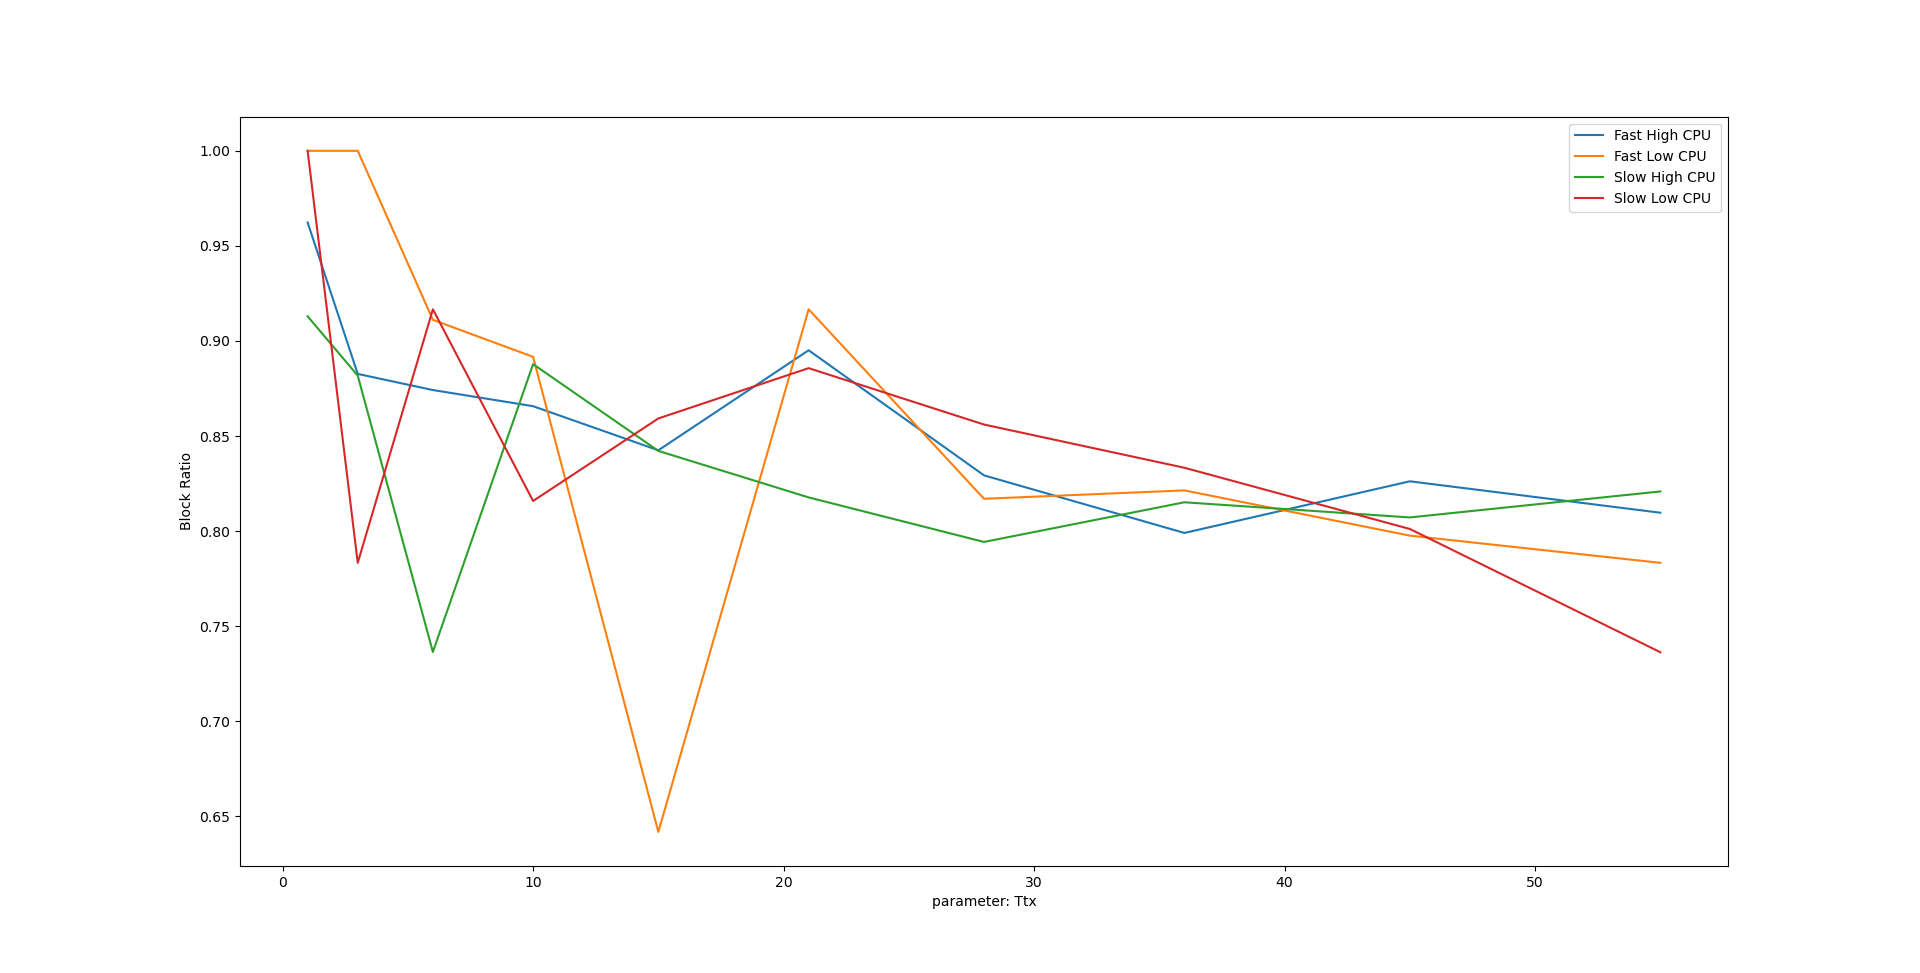
\includegraphics[width=0.8\textwidth]{../images/avg_run_3/Ttx.png}
		\caption{Ratio v/s Mean Transaction Interarrival Time}
		\label{fig:simulation_plot4}
	\end{figure}

	The above graph is the ratio vs the mean transaction interarrival time. Overall, the ratio shows a downwards trend as the mean transaction interarrival time increases. This is because the number of transactions produced in the network reduces, as the mean inter arrival time increases. So, the amount of overlap between various blocks (in terms of the transaction sets they contain) increases, and a larger fraction of blocks are declared to be invalid.

	\begin{figure}[H]
		\centering
		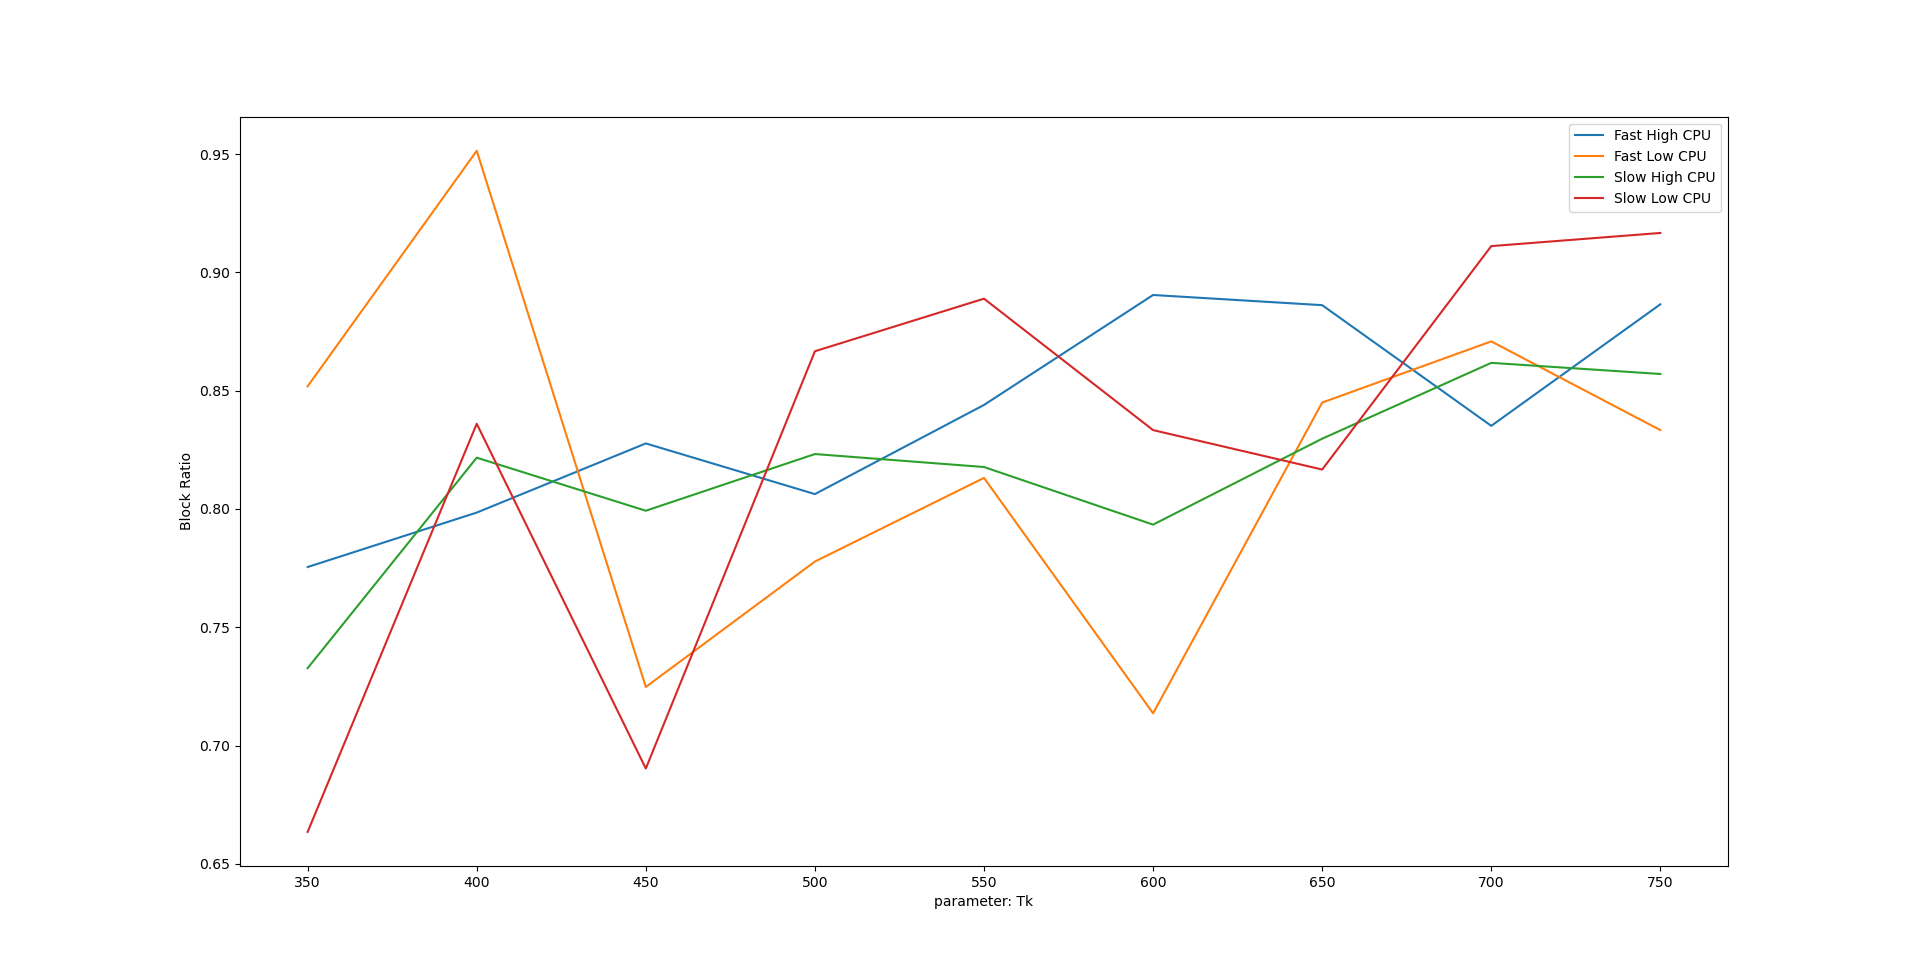
\includegraphics[width=0.8\textwidth]{../images/avg_run_3/Tk.png}
		\caption{Ratio v/s Mean Block Arrival Time}
		\label{fig:simulation_plot5}
	\end{figure}

	The above graph is the ratio vs the mean block arrival time. Overall, there is an upwards trend in the graph as the mean block arrival time increases. This is because the number of blocks produced in the network reduces, as the mean block arrival time increases. So, the amount of overlap between various blocks (in terms of the transaction sets they contain) decreases, and a smaller fraction of blocks are declared to be invalid.	
	
\end{solution}

\begin{solution}{Some sample blockchain trees}
	We will show the blockchain trees for the following set of parameters:

	\begin{itemize}
		\item Number of peers: 20 ; Percentage of slow peers: 50\% ; Percentage of low CPU peers: 50\% ; Mean transaction interarrival time: 10 seconds ; Mean block arrival time: 600 seconds ; Time of execution: 10 seconds
		\begin{figure}[H]
			\centering
			
\includegraphics[width=0.8\textwidth]{../images/b1.png}
		\end{figure}
		Here are the branch heights for the above tree:
		\begin{verbatim}
Branch Heights:- 33 42 42 48 50 52 64 64 66 93 104 106 106 107 108 110 110
		\end{verbatim}
		\item Number of peers: 20 ; Percentage of slow peers: 50\% ; Percentage of low CPU peers: 50\% ; Mean transaction interarrival time: 10 seconds ; Mean block arrival time: 6000 seconds ; Time of execution: 10 seconds
		\begin{figure}[H]
			\centering
			
\includegraphics[width=0.8\textwidth]{../images/b2.png}
		\end{figure}
		Here are the branch heights for the above tree:
		\begin{verbatim}
Branch Heights:- 32
		\end{verbatim}
		\item Number of peers: 20 ; Percentage of slow peers: 50\% ; Percentage of low CPU peers: 50\% ; Mean transaction interarrival time: 10 seconds ; Mean block arrival time: 6 seconds ; Time of execution: 10 seconds
		\begin{figure}[H]
			\centering
			
\includegraphics[width=0.8\textwidth]{../images/b3.png}
		\end{figure}

		Here are the branch heights for the above tree:
		\begin{verbatim}
Branch Heights:- 6 7 7 7 9 10 11 12 13 14 15 17 17 18 19 20 21 21 21 22 23 24
		\end{verbatim}
	\end{itemize}

	As we can see  that on varying the inter arrival block time, the number of branches in the tree also varies. For a very low block arrival time, the tree is very dense and has a lot of branches. For a very high block arrival time, the tree is very sparse and has very few branches.
	
\end{solution}

% \clearpage

\begin{solution}{Class Structure}
	\begin{figure}[H]
		\centering
		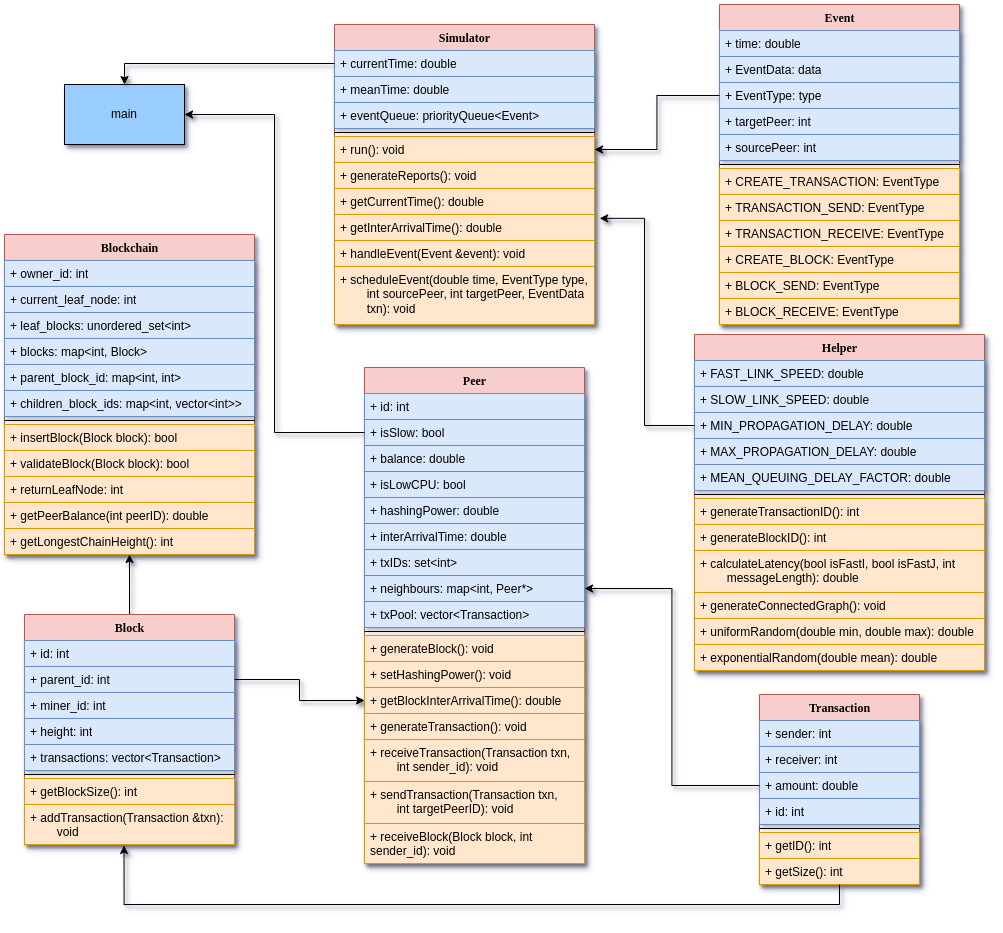
\includegraphics[width=0.8\textwidth]{../images/uml_class_coloured.png}
		\caption{Ratio v/s Mean Block Arrival Time}
		\label{fig:class-diagram}
	\end{figure}
\end{solution}

\begin{solution}{Simulator}
	\begin{itemize}
		\item The simulator calls the \texttt{run} function to start the simulation.
		\item It first calls the \texttt{generateConnectedGraph} function to create a connected graph of nodes.
		\item Each node then creates a genesis block using the \texttt{createGenesisBlock} function.
		\item The simulator schedules the creation of transactions by calling \texttt{scheduleEvent} with an inter-arrival time, event type, and node index.
	\end{itemize}
	
	\begin{mdframed}[linecolor=black, linewidth=2pt, roundcorner=10pt, backgroundcolor=yellow!10!white, skipabove=12pt, skipbelow=12pt]
	\begin{verbatim}
	void Simulator::run() {
		generateConnectedGraph();
		
		for (int i = 0 ; i < num_nodes ; i++ ) {
			peers[i]->createGenesisBlock();
		}
		
		for (int i = 0 ; i < num_nodes ; i ++ ) {
			double interArrivalTime = getInterArrivalTime();
			scheduleEvent(interArrivalTime, CREATE_TRANSACTION, i, -1, {});
		}
	}
	\end{verbatim}
	\end{mdframed}

	\begin{itemize}
		\item A random peer is selected to start mining by scheduling a \texttt{MINING\_START} event.
		\item The simulator processes events from the event queue by updating the current time and handling each event accordingly.
	\end{itemize}
	
	\begin{mdframed}[linecolor=black, linewidth=2pt, roundcorner=10pt, backgroundcolor=yellow!10!white, skipabove=12pt, skipbelow=12pt]
	\begin{verbatim}
		int random_peer = uniformRandom(0, num_nodes - 1);
		scheduleEvent(currentTime, MINING_START, random_peer, -1, {});
		while ( !eventQueue.empty() ) {
			Event current = eventQueue.top();
			eventQueue.pop();
			currentTime = current.time;
			handleEvent(current);
		}
	\end{verbatim}
	\end{mdframed}
	
\end{solution}

\begin{solution}{Transactions}
	A peer creates a transaction by calling the \texttt{generateTransaction} function.
	\begin{itemize}
		\item The peer checks its balance using the \texttt{getPeerBalance} function.
		\item If the balance is greater than zero, it selects a random target peer.
		\item A transaction is created and added to the transaction pool.
		\item The transaction is then broadcasted to all neighboring peers.
	\end{itemize}

\begin{mdframed}[linecolor=black, linewidth=2pt, roundcorner=10pt, backgroundcolor=yellow!10!white, skipabove=12pt, skipbelow=12pt]
	\begin{verbatim}
		void Peer::generateTransaction() {
			double our_balance = blockchain->getPeerBalance(id);
			if (our_balance <= 0) {
				return;
			}
			
			int targetPeerID = id;
			while (targetPeerID == id) {
				targetPeerID = uniformRandom(0, num_nodes - 1);
			}
			Transaction txn = Transaction(id, targetPeerID,uniformRandom(1, our_balance));
			txPool.insert(txn);
			for (auto& [id, peer] : neighbours) {
				sendTransaction(txn, peer->id);
			}
		}
	\end{verbatim}
\end{mdframed}

After the simulator first schedules the event \texttt{CREATE\_TRANSACTION} at each node:
    \begin{itemize}
        \item Each node generates a transaction and then a new time (\texttt{newTime}) is calculated by adding the current time to a value obtained from an exponential distribution using the function \texttt{getInterArrivalTime()}.
        \item The event \texttt{CREATE\_TRANSACTION} is then recursively scheduled on the same node with the newly calculated \texttt{newTime}.
    \end{itemize}

\begin{mdframed}[linecolor=black, linewidth=2pt, roundcorner=10pt, backgroundcolor=yellow!10!white, skipabove=12pt, skipbelow=12pt]
\begin{verbatim}
case CREATE_TRANSACTION:
	peers[event.sourcePeer]->generateTransaction();
	newTime = currentTime + getInterArrivalTime();
	scheduleEvent(newTime, CREATE_TRANSACTION, event.sourcePeer, -1, event.data);
	break;
	\end{verbatim}
\end{mdframed}
	
\end{solution}

\end{document}